%%%%%%%%%%%%%%%%%%%%%%%%%%%%%%%%%%%%%%%%%
% Programming/Coding Assignment
% LaTeX Template
%
% This template has been downloaded from:
% http://www.latextemplates.com
%
% Original author:
% Ted Pavlic (http://www.tedpavlic.com)
%
% Note:
% The \lipsum[#] commands throughout this template generate dummy text
% to fill the template out. These commands should all be removed when 
% writing assignment content.
%
% This template uses a Perl script as an example snippet of code, most other
% languages are also usable. Configure them in the "CODE INCLUSION 
% CONFIGURATION" section.
%
%%%%%%%%%%%%%%%%%%%%%%%%%%%%%%%%%%%%%%%%%

%----------------------------------------------------------------------------------------
%	PACKAGES AND OTHER DOCUMENT CONFIGURATIONS
%----------------------------------------------------------------------------------------

\documentclass{article}

\usepackage{fancyhdr} % Required for custom headers
\usepackage{lastpage} % Required to determine the last page for the footer
\usepackage{extramarks} % Required for headers and footers
\usepackage[usenames,dvipsnames]{color} % Required for custom colors
\usepackage{graphicx} % Required to insert images
\usepackage{listings} % Required for insertion of code
\usepackage{courier} % Required for the courier font
\usepackage{lipsum} % Used for inserting dummy 'Lorem ipsum' text into the template
\usepackage{setspace}
\usepackage{color}
\usepackage{comment}
\usepackage{caption}

\usepackage{hyperref}
\usepackage{natbib}
\usepackage{underscore}

\hypersetup{
    colorlinks=true,
    linkcolor=blue,
    filecolor=magenta,      
    urlcolor=cyan,
    breaklinks=true
}

%\usepackage[]{algorithm2e}
\usepackage{pdfpages}




%For python inclusion (http://widerin.org/blog/syntax-highlighting-for-python-scripts-in-latex-documents)
\definecolor{Code}{rgb}{0,0,0}
\definecolor{Decorators}{rgb}{0.5,0.5,0.5}
\definecolor{Numbers}{rgb}{0.5,0,0}
\definecolor{MatchingBrackets}{rgb}{0.25,0.5,0.5}
\definecolor{Keywords}{rgb}{0,0,1}
\definecolor{self}{rgb}{0,0,0}
\definecolor{Strings}{rgb}{0,0.63,0}
\definecolor{Comments}{rgb}{0,0.63,1}
\definecolor{Backquotes}{rgb}{0,0,0}
\definecolor{Classname}{rgb}{0,0,0}
\definecolor{FunctionName}{rgb}{0,0,0}
\definecolor{Operators}{rgb}{0,0,0}
\definecolor{Background}{rgb}{0.98,0.98,0.98}

% Margins
\topmargin=-0.45in
\evensidemargin=0in
\oddsidemargin=0in
\textwidth=6.5in
\textheight=9.0in
\headsep=0.25in

\linespread{1.1} % Line spacing

% Set up the header and footer
\pagestyle{fancy}
\lhead{\hmwkAuthorName} % Top left header
%\chead{\hmwkClass\ (\hmwkClassInstructor\ \hmwkClassTime): \hmwkTitle} % Top center head
\chead{\hmwkClass\ (\hmwkClassInstructor): \hmwkTitle} % Top center head
\rhead{\firstxmark} % Top right header
\lfoot{\lastxmark} % Bottom left footer
\cfoot{} % Bottom center footer
\rfoot{Page\ \thepage\ of\ \protect\pageref{LastPage}} % Bottom right footer
\renewcommand\headrulewidth{0.4pt} % Size of the header rule
\renewcommand\footrulewidth{0.4pt} % Size of the footer rule

\setlength\parindent{0pt} % Removes all indentation from paragraphs

%----------------------------------------------------------------------------------------
%	CODE INCLUSION CONFIGURATION
%----------------------------------------------------------------------------------------

\definecolor{MyDarkGreen}{rgb}{0.0,0.4,0.0} % This is the color used for comments
\lstloadlanguages{Perl} % Load Perl syntax for listings, for a list of other languages supported see: ftp://ftp.tex.ac.uk/tex-archive/macros/latex/contrib/listings/listings.pdf
\lstset{language=Perl, % Use Perl in this example
        frame=single, % Single frame around code
        basicstyle=\small\ttfamily, % Use small true type font
        keywordstyle=[1]\color{Blue}\bf, % Perl functions bold and blue
        keywordstyle=[2]\color{Purple}, % Perl function arguments purple
        keywordstyle=[3]\color{Blue}\underbar, % Custom functions underlined and blue
        identifierstyle=, % Nothing special about identifiers                                         
        commentstyle=\usefont{T1}{pcr}{m}{sl}\color{MyDarkGreen}\small, % Comments small dark green courier font
        stringstyle=\color{Purple}, % Strings are purple
        showstringspaces=false, % Don't put marks in string spaces
        tabsize=5, % 5 spaces per tab
        %
        % Put standard Perl functions not included in the default language here
        morekeywords={rand},
        %
        % Put Perl function parameters here
        morekeywords=[2]{on, off, interp},
        %
        % Put user defined functions here
        morekeywords=[3]{test},
       	%
        morecomment=[l][\color{Blue}]{...}, % Line continuation (...) like blue comment
        numbers=left, % Line numbers on left
        firstnumber=1, % Line numbers start with line 1
        numberstyle=\tiny\color{Blue}, % Line numbers are blue and small
        stepnumber=5 % Line numbers go in steps of 5
}

% Creates a new command to include a perl script, the first parameter is the filename of the script (without .pl), the second parameter is the caption
\newcommand{\perlscript}[2]{
\begin{itemize}
\item[]\lstinputlisting[caption=#2,label=#1]{#1.pl}
\end{itemize}
}


%----------------------------------------------------------------------------------------
%	DOCUMENT STRUCTURE COMMANDS
%	Skip this unless you know what you're doing
%----------------------------------------------------------------------------------------

% Header and footer for when a page split occurs within a problem environment
\newcommand{\enterProblemHeader}[1]{
\nobreak\extramarks{#1}{#1 continued on next page\ldots}\nobreak
\nobreak\extramarks{#1 (continued)}{#1 continued on next page\ldots}\nobreak
}

% Header and footer for when a page split occurs between problem environments
\newcommand{\exitProblemHeader}[1]{
\nobreak\extramarks{#1 (continued)}{#1 continued on next page\ldots}\nobreak
\nobreak\extramarks{#1}{}\nobreak
}

\setcounter{secnumdepth}{0} % Removes default section numbers
\newcounter{homeworkProblemCounter} % Creates a counter to keep track of the number of problems

\newcommand{\homeworkProblemName}{}
\newenvironment{homeworkProblem}[1][Problem \arabic{homeworkProblemCounter}]{ % Makes a new environment called homeworkProblem which takes 1 argument (custom name) but the default is "Problem #"
\stepcounter{homeworkProblemCounter} % Increase counter for number of problems
\renewcommand{\homeworkProblemName}{#1} % Assign \homeworkProblemName the name of the problem
\section{\homeworkProblemName} % Make a section in the document with the custom problem count
\enterProblemHeader{\homeworkProblemName} % Header and footer within the environment
}{
\exitProblemHeader{\homeworkProblemName} % Header and footer after the environment
}

\newcommand{\problemAnswer}[1]{ % Defines the problem answer command with the content as the only argument
\noindent\framebox[\columnwidth][c]{\begin{minipage}{0.98\columnwidth}#1\end{minipage}} % Makes the box around the problem answer and puts the content inside
}

\newcommand{\homeworkSectionName}{}
\newenvironment{homeworkSection}[1]{ % New environment for sections within homework problems, takes 1 argument - the name of the section
\renewcommand{\homeworkSectionName}{#1} % Assign \homeworkSectionName to the name of the section from the environment argument
\subsection{\homeworkSectionName} % Make a subsection with the custom name of the subsection
\enterProblemHeader{\homeworkProblemName\ [\homeworkSectionName]} % Header and footer within the environment
}{
\enterProblemHeader{\homeworkProblemName} % Header and footer after the environment
}

%----------------------------------------------------------------------------------------
%	NAME AND CLASS SECTION
%----------------------------------------------------------------------------------------

\newcommand{\hmwkTitle}{Assignment\ \#5 } % Assignment title
%\newcommand{\hmwkDueDate}{Monday,\ January\ 1,\ 2012} % Due date
\newcommand{\hmwkClass}{Introduction to Web Science} % Course/class
%\newcommand{\hmwkClassTime}{10:30am} % Class/lecture time
\newcommand{\hmwkClassInstructor}{Dr. Nelson} % Teacher/lecturer
\newcommand{\hmwkAuthorName}{Alexander Nwala} % Your name

%----------------------------------------------------------------------------------------
%	TITLE PAGE
%----------------------------------------------------------------------------------------

\title{
\vspace{2in}
\textmd{\textbf{\hmwkClass:\ \hmwkTitle}}\\
%\normalsize\vspace{0.1in}\small{Due\ on\ \hmwkDueDate}\\
%\vspace{0.1in}\large{\textit{\hmwkClassInstructor\ \hmwkClassTime}}
\vspace{0.1in}\large{\textit{\hmwkClassInstructor}}
\vspace{3in}
}

\author{\textbf{\hmwkAuthorName}}
\date{Thursday, October 16, 2014} % Insert date here if you want it to appear below your name

%----------------------------------------------------------------------------------------

\begin{document}

\maketitle



%----------------------------------------------------------------------------------------
%	TABLE OF CONTENTS
%----------------------------------------------------------------------------------------

%\setcounter{tocdepth}{1} % Uncomment this line if you don't want subsections listed in the ToC

\newpage
\tableofcontents
\newpage

%----------------------------------------------------------------------------------------
%	PROBLEM 1
%----------------------------------------------------------------------------------------

% To have just one problem per page, simply put a \clearpage after each problem

\begin{homeworkProblem}
The ``friendship paradox'' (\url{http://en.wikipedia.org/wiki/Friendship_paradox})
says that your friends have more friends than you do.  \\

Explore the friendship paradox for your Twitter account.  Since
Twitter has directional links (i.e., ``followers'' and ``following''),
we'll be investigating if the people you follow (Twitter calls these
people ``friends'') follow more people than you.  If you are following \textless 
50 people, use my twitter account ``phonedude_mln'' instead of your own.\\

Create a graph of the number of friends (y-axis) and the friends sorted
by number of friends (x-axis).  (The friends don't need to be labeled on
the x-axis as ``Bob'', ``Mary'', etc. -- just 1, 2, 3 ...)  In other words,
if you have 100 friends your x-axis will be 1..101 (100 + you), and the
y-axis value will be number of friends that each of those friends has.
The friend with the lowest number of friends will be first and the friend
with the highest number of friends will be last.\\

Do include yourself in the graph and label yourself accordingly.  Compute
the mean, standard deviation, and median of the number of friends that
your friends have.\\

The appropriate part of the Twitter API to use is:

\url{https://dev.twitter.com/rest/reference/get/friends/list}

%\lstinputlisting[breaklines=true, caption=Curl Demo]{"/home/anwala/CS 895/Assignment 1/problem1_curlDemonstration.py"}
%\lstinputlisting[breaklines=true, caption=Hash function; extract HTML funtion; and strip HTML tags function]{hashExtractProcessHTMlSnippet.py}


\begin{comment}
\begin{figure}
    \caption{curlDemoOutput}
    \begin{center}
        \includegraphics{curlDemo} % Example image
    \end{center}
\end{figure}
\end{comment}

%\problemAnswer
%{
    \begin{verbatim}\end{verbatim}
    \textbf{SOLUTION 1}\\

    The solution for this problem is outlined by the following steps:
    \begin{enumerate}

    \item \textbf{Establish connection between application and Twitter:} This was achieved through
    Tweepy \cite{Tweepy} which provides a python wrapper for the Twitter API.
    \item \textbf{Authenticate application:} This was achieved by registering the application and generating OAuth \cite{Oauth} access tokens.
    \item \textbf{Fetch all friends:} With the use of Dr. Nelson's Twitter account (phonedude_mln) and the Twitter user.friends() method, all friends were retrieved.
    \item \textbf{Fetch the count of friends of friends:} Finally, given the friends derived in the previous step, the user.friends_count() method was applied to get the count of friends of friends as outlined in Listing 1.

    \begin{verbatim}
        The file FoFCountTwitter.csv contains the 
        complete list of friends and their total friends count
    \end{verbatim}

    \lstinputlisting[breaklines=true, caption=Twitter: Get The Count Of Friends Of Friends]{getFoFSnippet.py}

    \end{enumerate}

    \begin{verbatim}\end{verbatim}
    \textbf{CONCLUSION 1}\\

    Based on Chart 1, it is clear that the friendship paradox holds; Dr. Nelson has less friends than his friends.

    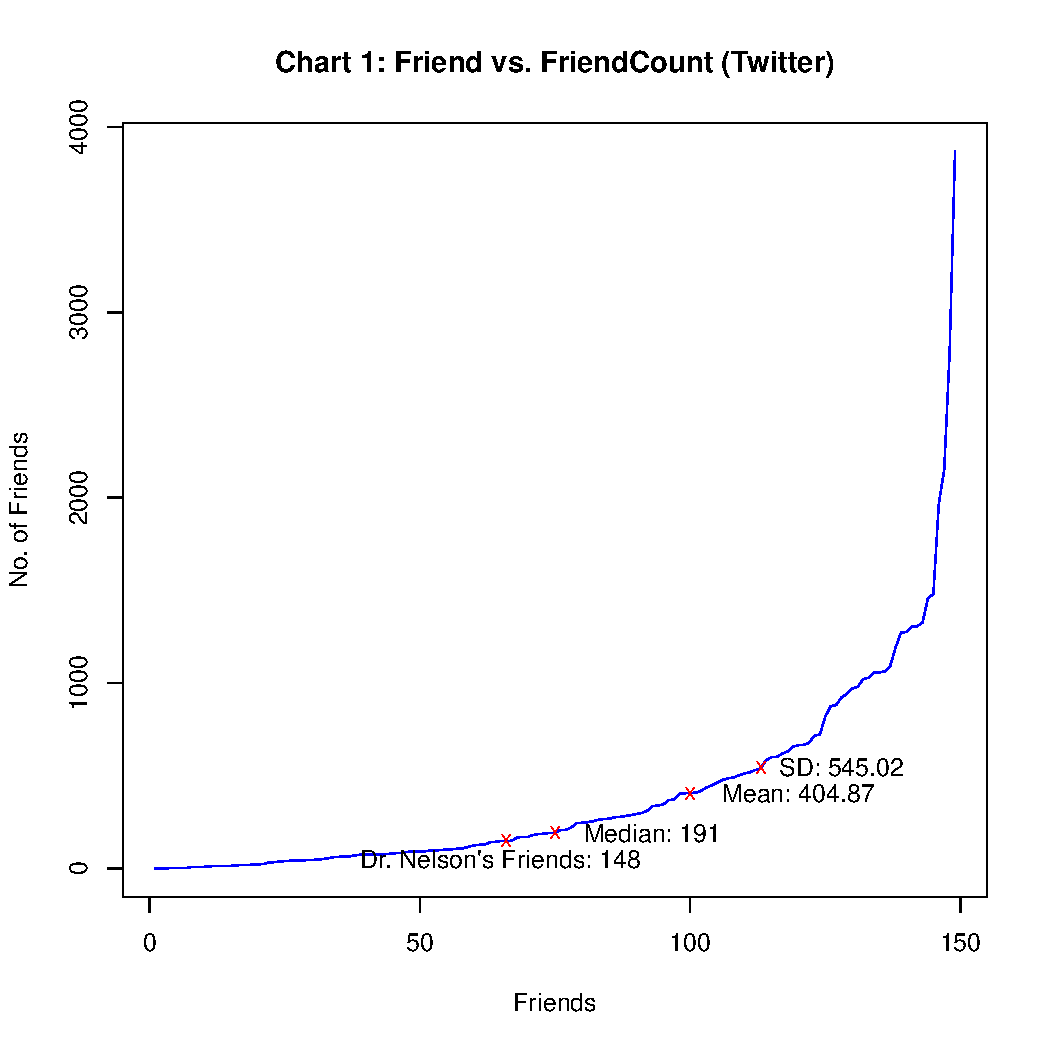
\includegraphics[width=\textwidth,scale=0.5]{/home/anwala/CS895/Assignment5/FoFCountTwitter.pdf}
    
%}



\end{homeworkProblem}

%----------------------------------------------------------------------------------------
%	PROBLEM 2
%----------------------------------------------------------------------------------------

\begin{homeworkProblem}
Using your facebook account, repeat question \#1 (if you have \textgreater 
50 friends).

Start at: \url{https://developers.facebook.com/docs/graph-api/reference/v2.1/user/friends}

or perhaps:

\url{http://socialnetimporter.codeplex.com/}
\begin{verbatim}\end{verbatim}
\textbf{SOLUTION 2}\\

The Facebook API restricts seeing the friends of friends; only the friends of people who use the Facebook API and have granted permission to the third-party application can be retrieved. Consequently, I used the Selenium \cite{Selenium} web browser automation/testing tool to retrieve the friends of my friends (the count) for those who share this information.

The solution for this problem is outlined by the following steps:
\begin{enumerate}
    \item \textbf{Login into Facebook:} Using my Facebook account, I was able to login into Facebook with selenium by supplying my credentials to the HTML username and password elements as outlined in Listing 2.

    \lstinputlisting[breaklines=true, caption=Facebook Login With Selenium]{loginToFacebookSnippet.py}

    \item \textbf{Open the friends page and scroll to the bottom of page:} Following authentication, the application subsequently opened my friends page (\url{https://www.facebook.com/friends/}). But since only a subset of my friends are viewable, the application scrolls to the end of the page in order to load all my friends data as outlined in Listing 3.

    \lstinputlisting[breaklines=true, caption=Scroll To the Bottom of my Friends Page]{fromFriendsPageScrollToBottomSnippet.py}

    \item \textbf{Download HTML content:} Having loaded all friends data, the application saves the html data into a file as outlined in Listing 3, Line 26.

    \item \textbf{Process HTML content to retrieve the count of the friends of my friends:} With the use of BeautifulSoup \cite{BeautifulSoup}, data of form\begin{verbatim}<friend, friendCount>\end{verbatim} was written into the file \textbf{FoFCountFacebook.csv} as outlined by Listing 4.

    \lstinputlisting[breaklines=true, caption=Facebook: Get The Count Of Friends Of Friends]{extractFoFfromHTMLSnippet.py}

    \begin{verbatim}\end{verbatim}
    \textbf{CONCLUSION 2}\\

    Based on Chart 2, it is clear that the friendship paradox holds; I have less friends than my friends.

    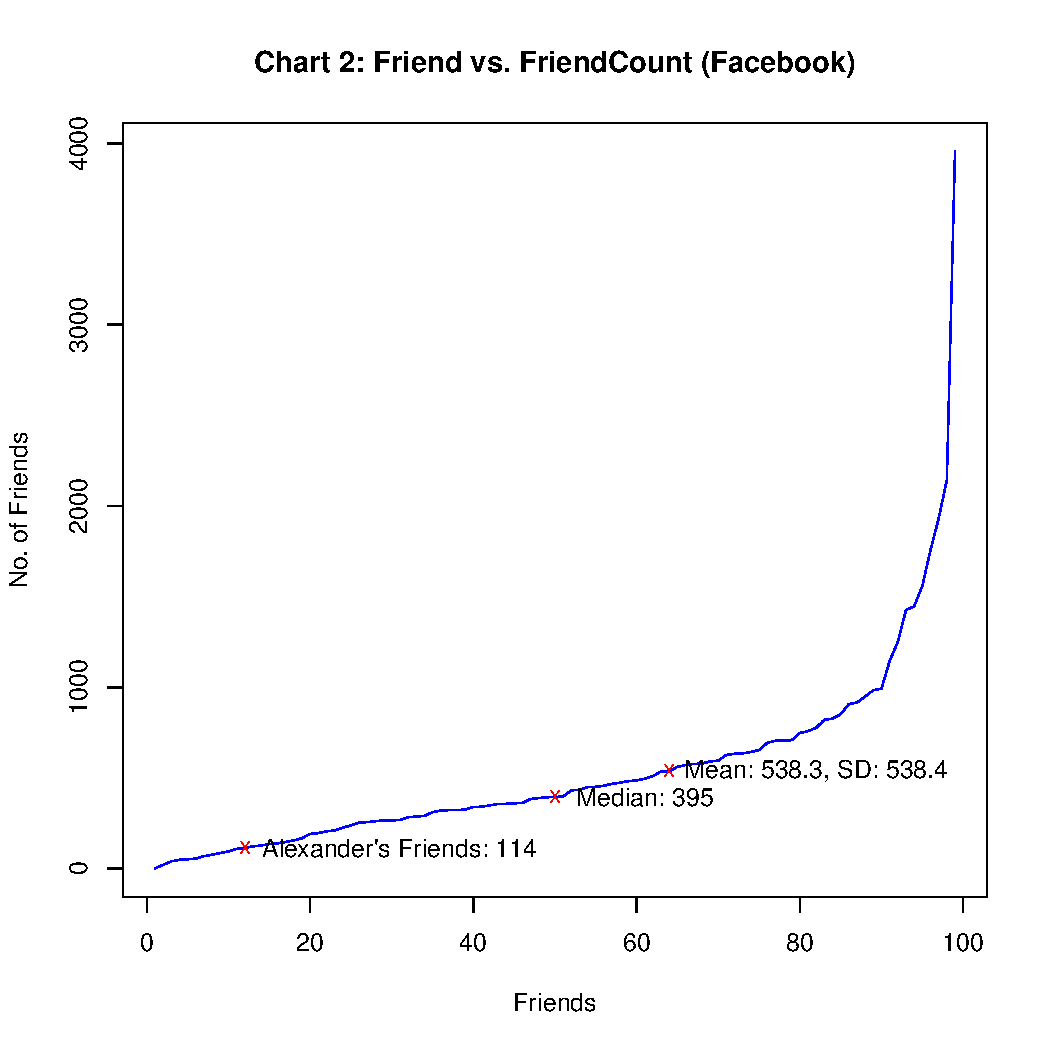
\includegraphics[width=\textwidth,scale=0.5]{/home/anwala/CS895/Assignment5/FoFCountFacebook.pdf}


\end{enumerate}



\begin{comment}
\begin{figure}
\caption{Uris distribution}
\begin{center}
    %\includegraphics{/home/anwala/CS895/Assignment2/urisDistribution.png} % Example image
    %\includepdf[pages={1},width=\textwidth,scale=0.5]{/home/anwala/CS895/Assignment2/Rplots.pdf}
\end{center}
\end{figure}
\end{comment}

\end{homeworkProblem}

%----------------------------------------------------------------------------------------
%   PROBLEM 3
%----------------------------------------------------------------------------------------
\begin{homeworkProblem}

Using your linkedin account, repeat question \#1 (if you have \textless
50 connections).

Start at: \url{https://developer.linkedin.com/apis}

\begin{verbatim} \end{verbatim}
\textbf{SOLUTION 3}\\

Similar to Facebook, the LinkedIn API restricts seeing the 2nd degree connections (friends of friends). Consequently, I used the Selenium web browser automation/testing tool to retrieve the 2nd degree connections (the count).

The solution for this problem is outlined by the following steps:
\begin{enumerate}

\item \textbf{Login into LinkedIn:} Using Jose Antonio Olvera Cañizares' account, I was able to login into LinkedIn with selenium by supplying my credentials to the HTML username and password elements as outlined in Listing 5.

\lstinputlisting[breaklines=true, caption=LinkedIn Login With Selenium]{loginToLinkedInSnippet.py}

\item \textbf{Open/download/process the Connections page:} Following authentication, the application subsequently opened Jose's Connections page (\url{https://www.linkedin.com/people/connections?trk=nav_responsive_tab_network}). This page was downloaded and serves as the initial input to retrieve 2nd degree connections as outlined in Listing 6. From this page, with the use of BeautifulSoup, the count of the connections of Jose's connection (2nd degree connection) were extracted as outlined in Listing 6.

\lstinputlisting[breaklines=true, caption=LinkedIn: Get The Count Of Friends Of Friends]{get2ndDegreeConnectionsSnippet.py}

\item \textbf{Dereference connections with 500+ connections:} connections who have more than 500 connections have there connections count expressed as 500+. Consequently, Listing 7 dereferences this 500+ link to get the exact number, for connections with over 500 connections. This was achieved by retrieving the HTML IDs of connections which fulfilled this criteria. Subsequently, with Selenium, a search query was submitted (Listing 7, Line 16), in order to retrieve the page which contains the exact number of connections. After dereferencing these, the result was appended to \textbf{FoFCountLinkedIn.csv}

\lstinputlisting[breaklines=true, caption=LinkedIn: Get The Count Of Friends Of Friends For Friends With 500+ Friends]{derefConnections.py}

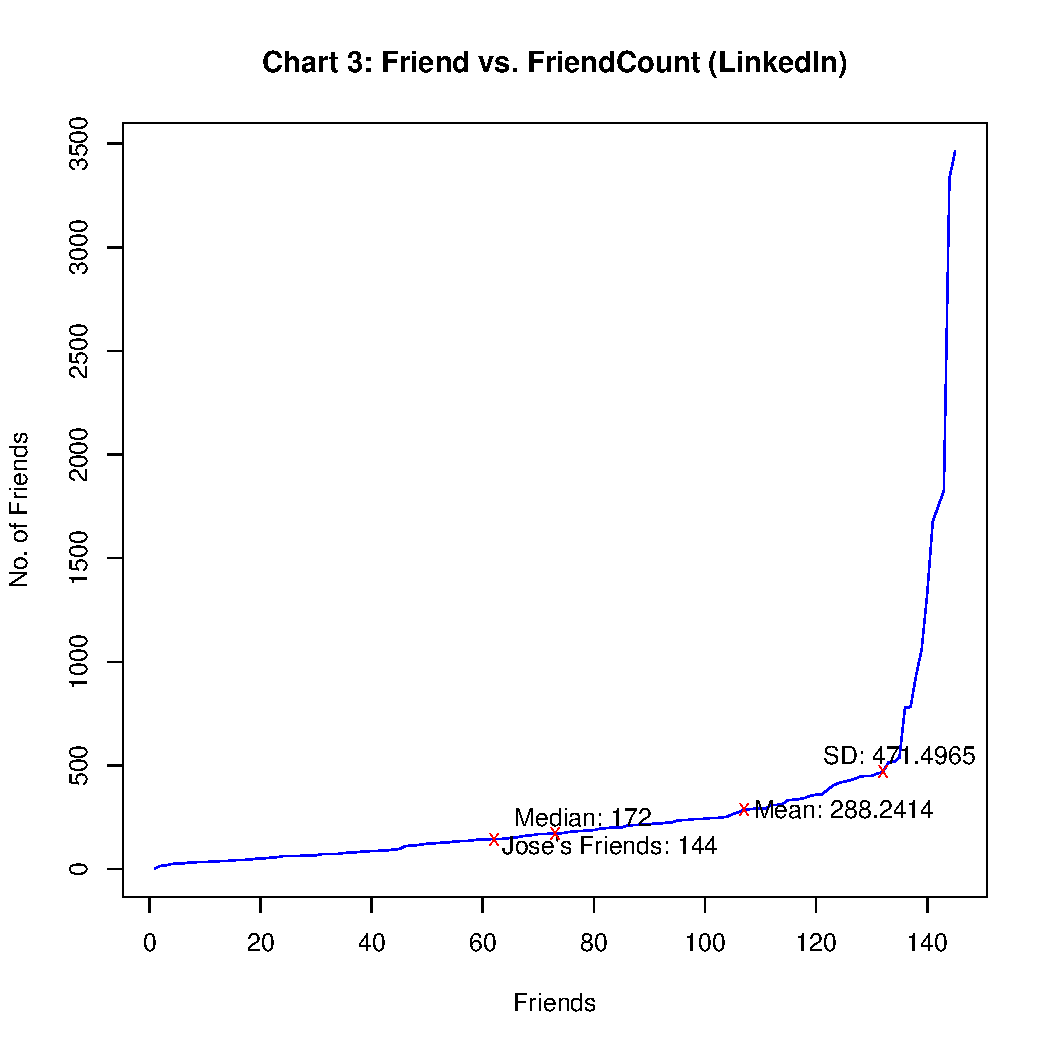
\includegraphics[width=\textwidth,scale=0.5]{/home/anwala/CS895/Assignment5/FoFCountLinkedIn.pdf}

\begin{verbatim}\end{verbatim}
\textbf{CONCLUSION 3}\\
Based on Chart 3, it is clear that the friendship paradox holds; Jose has less friends than his friends.

\end{enumerate}

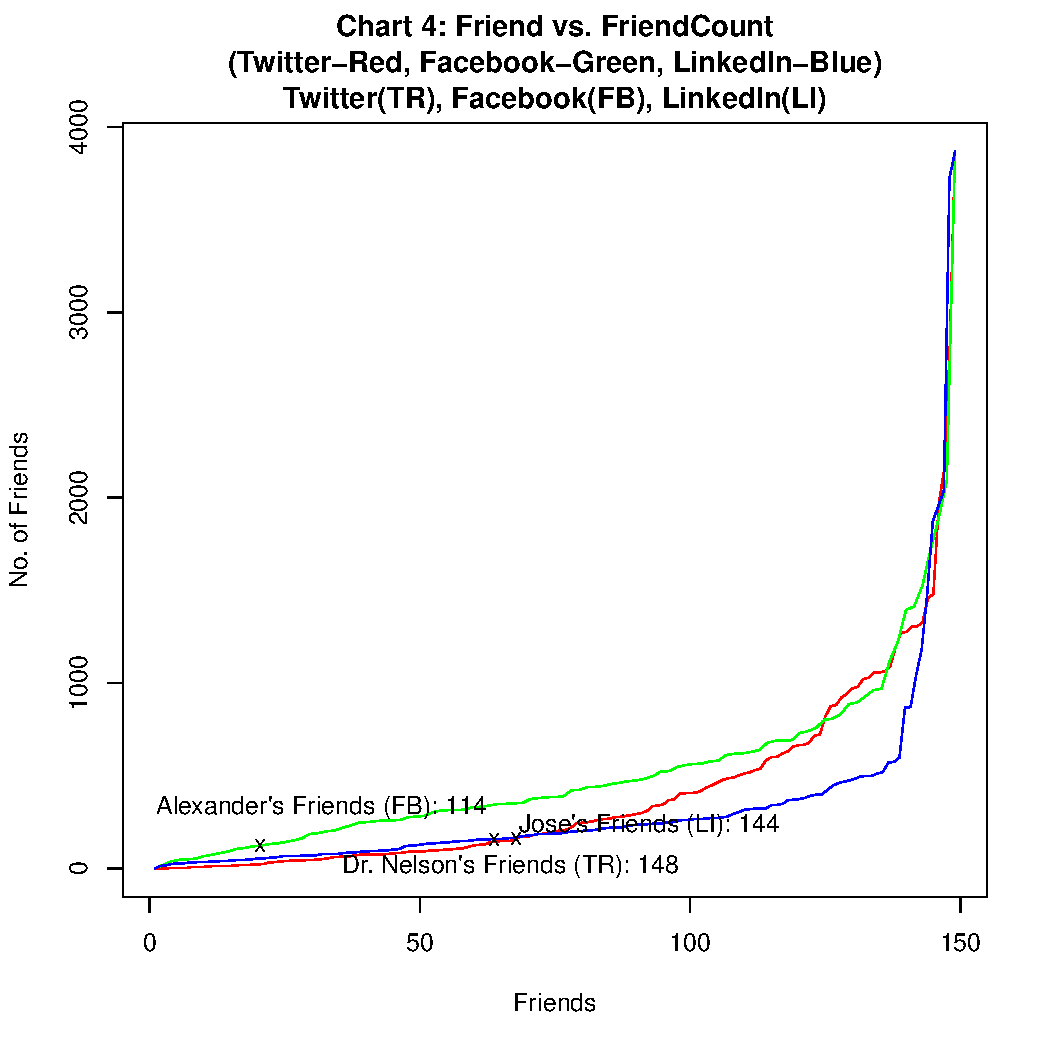
\includegraphics[width=\textwidth,scale=0.5]{/home/anwala/CS895/Assignment5/FoFCountCombined.pdf}

\end{homeworkProblem}
\begin{verbatim}\end{verbatim}



\bibliographystyle{plain}
\bibliography{A5bibFile}

%----------------------------------------------------------------------------------------

\end{document}